\documentclass[10p]{article} 
\usepackage[export]{adjustbox}
\usepackage{biblatex}
\usepackage{relsize}
\usepackage[ngerman]{babel}
\usepackage[a5paper,left=1.5cm,right=1.5cm,top=1cm,bottom=2cm]{geometry}
\usepackage{wrapfig}
\usepackage{graphicx}


\bibdata{uni.bib}
\bibliography{uni.bib}

\begin{document}
\title{Unipolarmotor Versuchserklärung}
\author{Daniel Renschler}
\maketitle
\pagenumbering{gobble}


\section*{Aufbau}
Man nehme ein Kupferdraht, einen Magneten, eine Schraube und eine Batterie. Magnet
wird auf den Kopf der Schraube gesetzt, und die Spitze der Schraube auf dem
Pluspol der Batterie angesetzt und an der Batterie angehoben, sodass die Schraube mit
Magnet in der Luft ist. Dann nehme man den Kupferdraht um Minuspol der Batterie
(am Magnet) mit dem Pluspol zu verbinden. Und siehe was passiert.
\section*{Erklärung}

%%Picture
\begin{wrapfigure}{r}{0.4\textwidth}
\centering
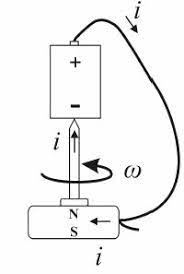
\includegraphics[width=.4\linewidth]{Unipolar1.jpeg}
\caption{Unipolarmotor \cite{assis2012ampere}}
\label{fig:wrapfig}
\end{wrapfigure}

Die Kräfte hier kann man sich am besten Vorstellen mit der "Rechten-Faust-Regel"
indem man seine rechte Hand bis auf den Daumen in ein Faust ballt und der Daumen
in die Stromrichtung zeigt (von + nach -), dann zeigen die Gekrümmten Finger die
Richtung der Mangetfeldlinien, welche die Schraube gegen den Uhrzeigersinn
rotieren (von der Batterie aus geschaut), solange Dauerstrom (i) von der
Batterie ausgeht und der Magnet Richtung Erde gerichtet ist. 


%%Bibliografie
\printbibliography

\end{document}
